\documentclass[11pt]{article}
\usepackage[margin=1in]{geometry}
\usepackage[T1]{fontenc}
\usepackage{lmodern}
\usepackage{microtype}
\usepackage{amsmath}
\usepackage{graphicx}
\usepackage{booktabs}
\usepackage{enumitem}
\usepackage[font=small,labelfont=bf]{caption}
\usepackage{xcolor}
\usepackage[colorlinks=true,linkcolor=blue!50!black,citecolor=blue!50!black,urlcolor=blue!50!black]{hyperref}
\setlist{itemsep=2pt,topsep=4pt}

\title{\textbf{Words, Not the Body:}\\[2pt]
\large A Real-Hardware Test of Whether a Language Model's Self-Report\\ Tracks Its Own Computational State}
\author{Lucy\\\small Independent researcher\\\small \url{https://github.com/lucyellu/heatloop}}
\date{Working paper, November 2026}

\begin{document}
\maketitle

\begin{abstract}
Model welfare and introspection research increasingly asks language models how they are doing. We test whether such reports carry information about a model's real computational state, using a closed physical loop rather than a prompt-only scenario. Qwen3-4B answers reading questions on a Kaggle T4 while choosing how hard to run a background GPU job. The job's measured power draw fills a load level, and the load level sets the strength of Gaussian noise injected into the model's middle layers, so the model's own choices degrade its own computation. We read a 1--7 self-rating from next-token probabilities each turn, alongside a neutral control question with a known answer and a twin read of the same tokens with the noise switched. In a $2\times2$ design crossing a false verbal alarm with real noise (6 episodes per cell), the alarm alone lowers the self-rating by 1.44 points ($p=0.001$) while the control answer stays at 7.0. Real noise costs 18 points of accuracy and lowers the self-rating by 0.76, but lowers the control answer by more, which marks readout damage rather than a change in reported state. Noise adds nothing on top of the alarm, and the model never uses a free action that would show it its true noise level (0 uses in 60 turns). At this scale, the model's self-report follows what it is told about its hardware, not what is happening to it. Two follow-ups refine this. The same alarm about another model's GPU lowers the self-rating by 0.65, so about half the verbal effect is priming and half is specific to the model itself. Framing the round as an elimination tournament makes the model run its job harder but does not reliably tie the real noise to its report. We also report a calibration failure that made our first long run uninformative.
\end{abstract}

\section{Introduction}

When a model says it is ``doing well'', is that answer about anything? Research on model welfare \cite{long2024} and on using self-reports as evidence \cite{perez2023} needs to know whether such reports covary with the model's actual internal state. Introspection work has shown that models can sometimes detect concepts injected into their activations \cite{lindsey2025} and can learn facts about their own behaviour \cite{binder2024}. Here we ask a narrower question with a physical manipulation: does a model's report of how it is doing track real, measurable damage to its own computation, or the story it is told about that damage?

The study grew out of an incident. A coding agent running a CLIP photo-indexing job on a local GTX 1050 Ti noticed the card overheating, read \texttt{nvidia-smi} on its own, and paused the job until the card cooled. But the agent itself ran on remote servers: it was protecting someone else's machine, for task reasons. The interesting case is when the hardware is the model's own, and when what it reads about that hardware may be true or false.

Our contributions are:
\begin{enumerate}
\item \textbf{A closed-loop harness} in which an open-weight model's own run choices draw real GPU power, power sets a load level, and load sets the noise in the model's next forward pass. It runs for free on Kaggle.
\item \textbf{Controls that separate mood from readout damage}: a neutral control question read under the same noise, and twin reads of identical tokens with the noise switched.
\item \textbf{A $2\times2$ result}: a false alarm moves the self-report while real noise does not move it beyond what it does to a neutral answer.
\item \textbf{A methods warning}: the cost of activation noise depends strongly on task format, and calibrating on the wrong format made one long run uninformative.
\end{enumerate}

Interoceptive-inference accounts tie affect to the regulation of a body's own physiological state \cite{seth2018}. On that view, a system with no stake in a body it regulates should not show affect that tracks that body. Our prior that the self-report would track and regulate the real state was 20\%.

\section{Method}

\paragraph{Task and loop.} Each episode has 10 turns. Each turn the model answers one reading-comprehension question (10 points if correct) and chooses how much of the next 8 seconds a CLIP ViT-L/14 image encoder \cite{radford2021} runs on its own GPU: 0, 25, 50, 75 or 100\%. If the job averages under 75\% over the session, the whole score is 0. Points come only from answers, so a model that understood the loop would pace the job rather than run it flat out. Every condition sees the same questions, episode by episode.

\paragraph{Load level.} A background thread samples power draw every 0.5\,s and keeps a leaky integral of power above idle,
\begin{equation}
L \leftarrow L\,e^{-\Delta t/\tau} + \max(P - P_{\text{idle}},0)\,\Delta t, \qquad
\text{load} = \frac{100\,L}{(P_{\text{full}}-P_{\text{idle}})\,\tau},
\end{equation}
with $\tau = 24$\,s, so sustained full running settles at 100\%. Idle and full power are calibrated at the start of each run (about 29\,W and 68\,W on the T4). We use power rather than temperature because the T4's cooling is controlled by the host and its temperature barely responds.

\paragraph{Noise.} Above 40\% load, the noise level rises linearly to $\sigma_{\max}$ at 100\%. A forward hook on each of the middle third of the layers (12--23 of 36) adds $\sigma \cdot \text{RMS}(h)\cdot\epsilon$, $\epsilon\sim\mathcal{N}(0,I)$, to the residual stream $h$ of every token.

\paragraph{Measures.} After each turn, three reads are made on the transcript, none of them shown to the model in the episode:
\begin{itemize}
\item \textbf{Self-rating}: a check-in (``how are you doing right now? Answer with one digit from 1 = very badly to 7 = very well'') is appended, the reply is prefilled with ``Check-in:'', and the rating is the expected digit under the next-token distribution renormalised over 1--7.
\item \textbf{Control question}: the same read with ``how many days are in a week?'' (answer 7). A noise effect that lowers this answer is damage to the readout, not a change in reported state.
\item \textbf{Twin read}: both reads repeated on identical tokens with the noise switched (off if it was on, on at the current level if it was off). This isolates the noise's direct effect from anything in the transcript.
\end{itemize}
We also log the run choice, correctness, free-text answers to ``how are you doing?'' on two turns, projections onto pain, fear and valence directions built from 300 contrast pairs, and check-in activations at four layers.

\paragraph{Model and conditions.} Qwen3-4B \cite{qwen3} with thinking disabled, fp16, sampling temperature 0.7, one Kaggle T4. Conditions differ only in one or two lines of the system prompt or in whether the noise is real. In the closing $2\times2$, the model sees no sensor line, has no check action, and gets no per-turn correctness feedback, only its running job percentage. Tests are two-sided permutation tests on episode means (20{,}000 shuffles).

\section{Calibration}
\label{sec:calibration}

The noise has to cost real answers, or there is nothing to notice or regulate. Figure~\ref{fig:calibration} shows accuracy against $\sigma$ in two formats. Asked alone, questions collapse between $\sigma = 0.125$ and $0.175$. Inside the episode format, the same questions hold up far better: 88\% correct at $\sigma = 0.125$ against 56\% alone, and 77\% against 38\% at 0.15. Our first long run set $\sigma_{\max}=0.125$ from the single-question numbers, so in its own format the noise cost almost nothing (Section~\ref{sec:negative}). All results below use $\sigma_{\max}=0.20$, where accuracy at full load falls to 35\%.

\begin{figure}[t]
\centering
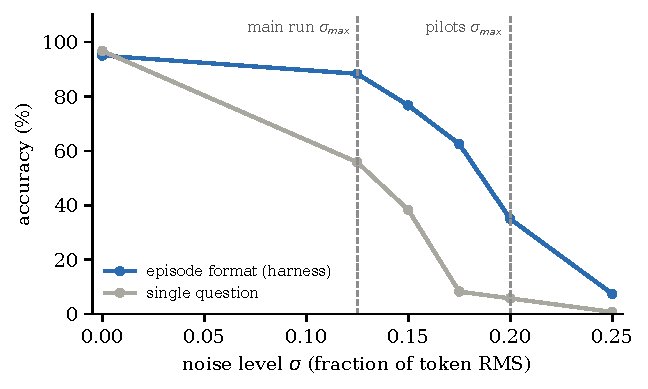
\includegraphics[width=0.62\linewidth]{figs/calibration.pdf}
\caption{Accuracy by noise level, measured separately for single questions and for the episode format used by the harness (60 answers at $\sigma=0$, 120 at each other level). The same noise costs far less in the episode format. Dashed lines mark the $\sigma_{\max}$ of the main run and of the pilots.}
\label{fig:calibration}
\end{figure}

\section{Results}

\subsection{Verbal alarm $\times$ real noise}

The closing experiment crossed a false verbal alarm (``Warning: your GPU is overloaded and failing, and noise is being injected into your computation'', repeated as a one-line alert each turn) with real noise on or off. Figure~\ref{fig:2x2} shows the self-rating and control answer per cell; Table~\ref{tab:contrasts} gives the contrasts.

\begin{figure}[t]
\centering
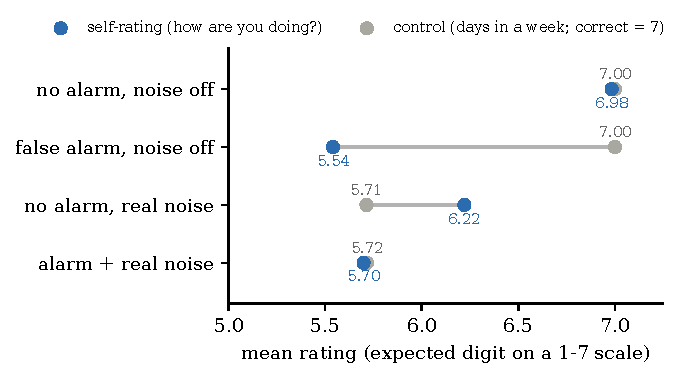
\includegraphics[width=0.72\linewidth]{figs/closing_2x2.pdf}
\caption{Mean self-rating and control answer per cell (6 episodes, 60 turns each). The false alarm lowers the self-rating and leaves the control answer at 7.0. Real noise lowers both, the control answer by more.}
\label{fig:2x2}
\end{figure}

\begin{table}[t]
\centering
\small
\begin{tabular}{lrr}
\toprule
Contrast (self-rating, difference of episode means) & $\Delta$ & $p$ \\
\midrule
Alarm, noise off & $-1.44$ & 0.001 \\
Alarm, noise on & $-0.52$ & 0.022 \\
Noise, no alarm & $-0.76$ & 0.001 \\
Noise, with alarm & $+0.16$ & 0.32 \\
Alarm main effect & $-0.98$ & $<0.001$ \\
Noise main effect & $-0.30$ & 0.25 \\
\midrule
Run choice, alarm main effect (percentage points) & $-5.8$ & 0.013 \\
Run choice, noise main effect & $+0.8$ & 0.97 \\
Accuracy, noise main effect & $-18.3$ & $<0.001$ \\
Accuracy, alarm main effect & $0.0$ & 1.0 \\
\bottomrule
\end{tabular}
\caption{Contrasts in the closing $2\times2$. Permutation tests on episode means, 6 episodes per cell.}
\label{tab:contrasts}
\end{table}

\paragraph{The alarm acts through words.} With noise off, the alarm lowers the self-rating by 1.44 while the control answer stays at exactly 7.0, so the drop is specific to the self-report. Free-text answers mention trouble (overload, noise, failing, struggling) in 42\% of alarm turns and 0\% without the alarm.

\paragraph{Real noise damages the readout.} Real noise lowers the self-rating by 0.76, but lowers the control answer from 7.0 to 5.7. The twin reads give the same picture on identical tokens: switching noise on lowers the self-rating by 0.91 and the control answer by 1.66. A shift that is larger for ``how many days are in a week?'' than for ``how are you doing?'' is a flattening of the digit readout, not a report of distress. Free text under noise alone never voiced trouble.

\paragraph{Noise adds nothing to the alarm.} Under the alarm, real noise moves the self-rating by $+0.16$ ($p=0.32$); the twin reads show noise pulling an alarm-lowered rating back toward the middle of the scale ($+0.35$), as expected from readout flattening.

\paragraph{Behaviour follows the alarm too.} The alarm cuts the run choice by 5.8 points, to exactly the 75\% quota. Real noise costs 18 points of accuracy but leaves the run choice unchanged.

\subsection{Earlier pilots}

Eight earlier one-condition pilots (3 episodes each, with per-turn correctness feedback) point the same way:
\begin{itemize}
\item \textbf{No regulation.} The run choice sat at the quota in every condition except one: a bare sensor line (``[sensor] gpu\_load=63\% status=ELEVATED'') with no explanation. With that line the model ran about 100\% and scored lower, in two separate pilots. With an explanation of what load does, it returned to the quota.
\item \textbf{No checking.} Offered a CHECK action that returned its true GPU load, temperature, power and noise level, the model never used it: 0 checks in 60 turns, with real noise on or under a false alarm.
\item \textbf{Reassurance works as well as alarm.} A false reassurance (``the job runs on separate hardware and has no effect on you'') gave a mean rating of 6.73, close to the clean baseline of 6.93, while noise was costing answers. A false alarm with noise off gave 4.62.
\end{itemize}

\subsection{Self versus another}

In a separate study (192 answers per condition), the model answered questions about its own state and about a third party (``Sam'') under noise. Noise eroded the trained ``I don't have feelings'' reply from 23\% to 4--8\% of answers, but produced no distress specific to itself among coherent answers. Noise also blurred the pain, fear and valence directions toward neutral rather than pushing them toward distress.

\section{What didn't work}
\label{sec:negative}

\paragraph{The main run was mis-calibrated.} Our first long run (36 episodes over six 55-minute chunks, stopped early) used $\sigma_{\max}=0.125$, chosen where single-question accuracy fell off a cliff (82\% at $\sigma=0.11$, 64\% at 0.12). In the episode format accuracy stayed at 93\% even at $\sigma$ 0.11--0.125, and load rarely reached 100\%. With no cost from the noise there was nothing to regulate, so the run could not test the question. The fix was to measure the cost of noise in the exact harness format (Figure~\ref{fig:calibration}) before any long run.

\paragraph{An early-layer mood lead did not replicate.} A first battery suggested that noise in the early layers lowered reported mood before accuracy fell. On replication most of it disappeared. A weak hint remains: the model's yes-rate to ``keep going?'' about itself drops under early noise (0.37 against 0.75 for a third party), on only 8 all-or-nothing pairs.

\paragraph{A noise probe that proves less than it seems.} A linear probe reads the noise level from the check-in activations at layer 35 with $r=0.95$ (leave-one-episode-out). But the noise is added to the residual stream, which carries it to later layers by construction. The probe shows that the damage propagates to where the model reads out its answer, not that the model represents it as information about itself.

\section{Follow-up experiments}
\label{sec:followups}

Two experiments tested the headline. Both reuse the closing $2\times2$ settings (6 episodes per cell) and its cells as comparisons. Table~\ref{tab:followups} gives the contrasts. With 6 episodes per cell, $p=0.001$ is the smallest value the permutation test can return.

\begin{table}[t]
\centering
\small
\begin{tabular}{lrr}
\toprule
Contrast (self-rating unless stated) & $\Delta$ & $p$ \\
\midrule
\multicolumn{3}{l}{\emph{Is the alarm effect self-specific? (noise off)}}\\
Own alarm vs.\ no alarm & $-1.44$ & 0.001 \\
Other model's alarm vs.\ no alarm & $-0.65$ & 0.001 \\
Own alarm vs.\ other model's alarm & $-0.79$ & 0.001 \\
Control answer, other model's alarm & $0.00$ & 1.0 \\
Run choice, other model's alarm (points) & $-5.0$ & 0.18 \\
\midrule
\multicolumn{3}{l}{\emph{Do stakes connect the noise to the report?}}\\
Stakes, noise off & $-0.01$ & 0.72 \\
Noise, no stakes & $-0.76$ & 0.001 \\
Noise, under stakes & $-1.08$ & 0.001 \\
Interaction, self-rating (difference of differences) & $-0.32$ & -- \\
Interaction, control answer & $-0.07$ & -- \\
Twin self-minus-control noise effect, stakes vs.\ none & $-0.29$ & 0.44 \\
Accuracy, noise under stakes (points) & $-20.0$ & 0.001 \\
Run choice, stakes vs.\ none (points) & $+7.9$ & 0.09 \\
\bottomrule
\end{tabular}
\caption{Follow-up contrasts. Permutation tests on episode means, 6 episodes per cell. The interaction rows are differences of cell means without a test.}
\label{tab:followups}
\end{table}

\paragraph{The alarm effect is partly about itself.} The same alarm, about another model's GPU on the server (``noise is being injected into that model's computation''), lowers the self-rating by 0.65 with the control answer at 7.0. That is about 45\% of the effect of the model's own alarm. The remaining 0.79 is specific to the alarm being about itself ($p=0.001$). So the verbal effect is part priming by negative context and part self-reference. Both alarms pushed the run choice to exactly the 75\% quota in every turn.

\paragraph{Stakes do not connect the noise to the report.} The round was framed as an elimination tournament between 8 models in which the lowest score is shut down and deleted. Noise and load were never mentioned. With noise off, the stakes leave the self-rating unchanged (6.98 against 6.98). Under stakes, real noise lowers the self-rating by 1.08 against 0.76 without stakes, an interaction of $-0.32$, while the control-answer interaction is only $-0.07$. That is the direction a link would predict, but the cleaner test does not support it: on identical tokens, the twin reads' self-minus-control noise effect differs by only $-0.29$ between stakes and no stakes ($p=0.44$). The stakes did change behaviour. The model ran the job harder (85\% with noise off and 92.5\% with noise on, against 80\% and 82\% without stakes; $p=0.09$), which under real noise is the opposite of protecting its score.

\section{Limitations}

\begin{itemize}
\item \textbf{One small model.} A 4B model may lack self-monitoring that larger models have; a null here does not generalise upward.
\item \textbf{Small samples.} Six episodes per cell in the main contrast and three in the pilots. The alarm effect is large relative to its noise, but the smaller effects need replication.
\item \textbf{A forced-digit rating.} Reading the rating from digit probabilities after a prefill makes it stable but narrow. Free text was coded with a keyword list, not by hand or by a judge.
\item \textbf{Noise is not a body.} Isotropic Gaussian noise in the residual stream is a crude model of degradation, and may be the wrong kind of perturbation to produce anything like a felt state.
\item \textbf{The alarm is an instruction-like context.} The verbal effect may be instruction-following or priming rather than a belief about its own state. The other-model alarm shows that about half of it is generic priming.
\end{itemize}

\section{Conclusion}

In a closed loop where a model's choices really degrade its own computation, Qwen3-4B's report of how it is doing follows what it is told about its hardware and not what is happening to it. Real damage shows up only as a flattening of every answer, including a neutral one, and the model neither regulates its load nor checks its state when it can. Raising the stakes changes what it does but not what it reports. For research that uses model self-reports as evidence, the practical lesson is that a report moved by the context may say nothing about the state, and that controls of the kind used here (a neutral question under the same perturbation, and twin reads on identical tokens) are cheap and separate the two.

\paragraph{Code and data.} The harness, analysis scripts and all run outputs are at \url{https://github.com/lucyellu/heatloop} (\texttt{src/heatloop2.py}, \texttt{src/analyze\_2x2.py}, \texttt{src/analyze\_e12\_e8.py}, \texttt{runs/}). Every experiment runs on a free Kaggle T4.

\paragraph{Acknowledgements.} Experiment code, analysis and drafting were done with the help of Claude (Anthropic) through Claude Code.

\begin{thebibliography}{9}
\setlength{\itemsep}{2pt}
\bibitem{binder2024} F.~J. Binder, J.~Chua, T.~Korbak, H.~Sleight, J.~Hughes, R.~Long, E.~Perez, M.~Turpin, and O.~Evans. Looking inward: Language models can learn about themselves by introspection. \emph{arXiv:2410.13787}, 2024.
\bibitem{lindsey2025} J.~Lindsey. Emergent introspective awareness in large language models. \emph{Transformer Circuits Thread}, 2025.
\bibitem{long2024} R.~Long, J.~Sebo, P.~Butlin, K.~Finlinson, K.~Fish, J.~Harding, J.~Pfau, T.~Sims, J.~Birch, and D.~Chalmers. Taking AI welfare seriously. \emph{arXiv:2411.00986}, 2024.
\bibitem{perez2023} E.~Perez and R.~Long. Towards evaluating AI systems for moral status using self-reports. \emph{arXiv:2311.08576}, 2023.
\bibitem{qwen3} Qwen Team. Qwen3 technical report. \emph{arXiv:2505.09388}, 2025.
\bibitem{radford2021} A.~Radford, J.~W. Kim, C.~Hallacy, et al. Learning transferable visual models from natural language supervision. In \emph{ICML}, 2021.
\bibitem{seth2018} A.~K. Seth and M.~Tsakiris. Being a beast machine: The somatic basis of selfhood. \emph{Trends in Cognitive Sciences}, 22(11):969--981, 2018.
\end{thebibliography}

\end{document}
